The article prints the seven tables a reader needs to follow its argument.
This section carries the ones it summarises: the exclusion ledger, the
construct audit, the surface denominator, the planned contrasts, the region
labels, the ITSM family split, the sign-flip attribution, the cohort
decomposition, the axis-kind partition, the specification-curve comparison,
the desk utility, the tipping curve, the decision-curve corpus, the declared
measures, the four decision rules, the calibration diagnostics, the
availability evidence, the severity sweeps, the absorption ladders, and the
simulation in full. Every one is generated by
\texttt{scripts/make\_numbers.py} from the result files, and none is typed by
hand.

\subsection{The corpus}

\begin{table}[t]
\centering
\small
\resizebox{\ifdim\width>\linewidth\linewidth\else\width\fi}{!}{%%
\begin{tabular}{llll}
\toprule
log & domain & code & detail \\
\midrule
Helpdesk & itsm & NO\_HEADROOM & handover/primary prev=0.9993 \\
Helpdesk & itsm & NO\_HEADROOM & handover/g=workgroup prev=0.0011 \\
BPIC13\_open & itsm & SMALL\_N & n=819 \\
BPIC13\_closed & itsm & NO\_TEST\_VARIATION & duration \\
BPIC12 & lending & NO\_G & n=13087 \\
BPIC17 & lending & NO\_HEADROOM & handover/primary prev=0.9977 \\
BPIC19 & procurement & NO\_HEADROOM & handover/primary prev=0.9631 \\
BPIC15\_2 & permitting & SMALL\_N & n=832 \\
BPIC15\_5 & permitting & NO\_HEADROOM & handover/primary prev=0.9593 \\
BPIC20\_domestic & expenses & NO\_G & n=10500 \\
BPIC20\_intl & expenses & NO\_G & n=6449 \\
BPIC20\_prepaid & expenses & NO\_G & n=2099 \\
BPIC20\_permit & expenses & NO\_G & n=7065 \\
BPIC20\_rfp & expenses & NO\_G & n=6886 \\
Sepsis & healthcare & NO\_HEADROOM & handover/primary prev=1.0000 \\
HospitalBilling & healthcare & NO\_F & n=100000 \\
RoadFines & enforcement & NO\_HEADROOM & handover/primary prev=0.0037 \\
BPIC11 & healthcare & HELD\_OUT & downloaded as a held-out log for the out-of-corpus test; never offered to the admission rules \\
BPIC18 & agriculture & NO\_TEST\_VARIATION & held-out set: duration \\
BPIC18 & agriculture & NO\_HEADROOM & held-out set: handover prev=1.0000 \\
\bottomrule
\end{tabular}%
}
\caption{Every downloaded log that is not among the \nPairs\ admitted log--target pairs, with its registered exclusion code. \textsf{HELD\_OUT} names the logs downloaded as a held-out set for a separate test and never offered to the admission rules; every other code is a rule of Section~\ref{sec:design}. Some logs appear here under one target and among the admitted pairs under the other, which is what a per-pair admission rule does.}
\label{tab:corpus}
\end{table}


\begin{table}[t]
\centering
\footnotesize
\setlength{\tabcolsep}{5pt}%
\renewcommand{\arraystretch}{1.15}%
\hyphenpenalty=50 \exhyphenpenalty=50 \emergencystretch=1em\relax%
\resizebox{\ifdim\width>\linewidth\linewidth\else\width\fi}{!}{%%
\begin{tabular}{lllll>{\raggedright\arraybackslash}p{0.200\linewidth}>{\raggedright\arraybackslash}p{0.200\linewidth}}
\toprule
log & domain & target & register & free field & why it behaves as a register & threat to construct validity \\
\midrule
RoadFines & enforcement & duration & article & org:resource & article of law, reused across fines & semantics legal, not operational \\
Sepsis & healthcare & duration & Diagnose & org:group & diagnosis vocabulary: reused, not maintained & no maintenance process; quality axis hypothetical \\
BPIC13\_closed & itsm & handover & product & org:resource & maintained CI or customer register & none beyond domain: closest to the case study \\
BPIC13\_incidents & itsm & duration & product & org:resource & maintained CI or customer register & none beyond domain: closest to the case study \\
BPIC13\_incidents & itsm & handover & product & org:resource & maintained CI or customer register & none beyond domain: closest to the case study \\
BPIC14 & itsm & duration & CI Name (aff) & assignment group & maintained CI or customer register & none beyond domain: closest to the case study \\
BPIC14 & itsm & handover & CI Name (aff) & assignment group & maintained CI or customer register & none beyond domain: closest to the case study \\
Helpdesk & itsm & duration & customer & Resource & maintained CI or customer register & none beyond domain: closest to the case study \\
UCI498 & itsm & duration & caller\_id & assigned\_to & maintained CI or customer register & none beyond domain: closest to the case study \\
UCI498 & itsm & handover & caller\_id & assigned\_to & maintained CI or customer register & none beyond domain: closest to the case study \\
BPIC17 & lending & duration & case:RequestedAmount & org:resource & application or offer reference & near-unique per case, so reuse is thin \\
BPIC15\_1 & permitting & duration & case:parts & org:resource & case-type reference, reused & nobody curates it \\
BPIC15\_1 & permitting & handover & case:parts & org:resource & case-type reference, reused & nobody curates it \\
BPIC15\_3 & permitting & duration & case:parts & org:resource & case-type reference, reused & nobody curates it \\
BPIC15\_3 & permitting & handover & case:parts & org:resource & case-type reference, reused & nobody curates it \\
BPIC15\_4 & permitting & duration & case:parts & org:resource & case-type reference, reused & nobody curates it \\
BPIC15\_4 & permitting & handover & case:parts & org:resource & case-type reference, reused & nobody curates it \\
BPIC15\_5 & permitting & duration & case:parts & org:resource & case-type reference, reused & nobody curates it \\
BPIC19 & procurement & duration & case:Vendor & org:resource & item or vendor catalogue entry & target is a duration, not a routing decision \\
\bottomrule
\end{tabular}%
}
\caption{Construct validity, per log--target pair: the field playing the register role, why it behaves as a maintained and reused entity, the free field, and the specific threat to construct validity the pair carries. These are not the same construct, which is why the corpus is a benchmark of specification sensitivity rather than a replication.}
\label{tab:construct}
\end{table}


\begin{table}[t]
\centering
\small
\resizebox{\ifdim\width>\linewidth\linewidth\else\width\fi}{!}{%%
\begin{tabular}{lllllllllllllllr}
\toprule
log & target & learners & splits & quality & rungs & metrics & declared scalar & computed scalar & model fits & duplicates & missing & inference cells & draws & register levels K & K / n train \\
\midrule
BPIC13\_closed & handover & 2 & 6 & 6 & 3 & 5 & 1080 & 1080 & 288 & 0 & 0 & 36 & 400 & 337 & 0.324 \\
BPIC13\_incidents & duration & 2 & 6 & 6 & 3 & 5 & 1080 & 1080 & 288 & 0 & 0 & 36 & 400 & 704 & 0.133 \\
BPIC13\_incidents & handover & 2 & 6 & 6 & 3 & 5 & 1080 & 1080 & 288 & 0 & 0 & 36 & 400 & 704 & 0.133 \\
BPIC14 & duration & 4 & 6 & 10 & 4 & 5 & 4800 & 4800 & 1200 & 0 & 0 & 36 & 400 & 3019 & 0.093 \\
BPIC14 & handover & 4 & 6 & 10 & 4 & 5 & 4800 & 4800 & 1200 & 0 & 0 & 36 & 400 & 3019 & 0.093 \\
BPIC15\_1 & duration & 2 & 6 & 6 & 3 & 5 & 1080 & 1080 & 288 & 0 & 0 & 36 & 400 & 89 & 0.106 \\
BPIC15\_1 & handover & 2 & 6 & 6 & 3 & 5 & 1080 & 1080 & 288 & 0 & 0 & 36 & 400 & 89 & 0.106 \\
BPIC15\_3 & duration & 2 & 6 & 6 & 3 & 5 & 1080 & 1080 & 288 & 0 & 0 & 36 & 400 & 94 & 0.095 \\
BPIC15\_3 & handover & 2 & 6 & 6 & 3 & 5 & 1080 & 1080 & 288 & 0 & 0 & 36 & 400 & 94 & 0.095 \\
BPIC15\_4 & duration & 2 & 6 & 6 & 3 & 5 & 1080 & 1080 & 288 & 0 & 0 & 36 & 400 & 53 & 0.072 \\
BPIC15\_4 & handover & 2 & 6 & 6 & 3 & 5 & 1080 & 1080 & 288 & 0 & 0 & 36 & 400 & 53 & 0.072 \\
BPIC15\_5 & duration & 2 & 6 & 6 & 3 & 5 & 1080 & 1080 & 288 & 0 & 0 & 36 & 400 & 107 & 0.132 \\
BPIC17 & duration & 2 & 6 & 6 & 3 & 5 & 1080 & 1080 & 288 & 0 & 0 & 36 & 400 & 701 & 0.032 \\
BPIC19 & duration & 3 & 6 & 6 & 3 & 5 & 1620 & 1620 & 432 & 0 & 0 & 36 & 400 & 1975 & 0.011 \\
Helpdesk & duration & 2 & 6 & 6 & 3 & 5 & 1080 & 1080 & 288 & 0 & 0 & 36 & 400 & 394 & 0.123 \\
RoadFines & duration & 3 & 6 & 6 & 3 & 5 & 1620 & 1620 & 432 & 0 & 0 & 36 & 400 & 66 & 0.001 \\
Sepsis & duration & 2 & 6 & 6 & 3 & 5 & 1080 & 1080 & 288 & 0 & 0 & 36 & 400 & 147 & 0.200 \\
UCI498 & duration & 2 & 6 & 6 & 3 & 5 & 1080 & 1080 & 288 & 0 & 0 & 36 & 400 & 5245 & 0.301 \\
UCI498 & handover & 2 & 6 & 6 & 3 & 5 & 1080 & 1080 & 288 & 0 & 0 & 36 & 400 & 5245 & 0.301 \\
\bottomrule
\end{tabular}%
}
\caption{The surface denominator audit. For every log--target pair: the declared level count on each axis, then two counts \emph{on the same basis} --- the admissible scalar cells the declaration multiplies out, and the same cells counted in the surface file --- which are equal on every pair. `model fits' is a different quantity and is printed separately: it counts fitted arms before the expansion over instruments and \emph{includes} the intercept-only rung, which the master surface carries so that the surface is complete and which no admissible set contains. Then duplicates, missing combinations, the size and draw count of the inference surface, the register's cardinality and its ratio to the training row count, which Section~\ref{sec:simsensitivity} shows is what governs whether the bands cover at their nominal level.}
\label{tab:denominator}
\end{table}


\begin{table}[t]\centering\small
\textbf{??} this table's source has not been generated yet.
\caption{Confirmatory contrasts.}\label{tab:confirm}\end{table}


\subsection{Regions, sign flips and the cohort decomposition}

\begin{table}[t]
\centering
\small
\resizebox{\ifdim\width>\linewidth\linewidth\else\width\fi}{!}{%%
\begin{tabular}{llllllrlrl}
\toprule
log & target & cells & beneficial & harmful & unresolved & rho & region & q & label under the narrow family \\
\midrule
BPIC13\_closed & handover & 180 & 0 & 1 & 179 & -0.006 & conditionally harmful & 3.338 & sign-changing \\
BPIC13\_incidents & duration & 180 & 21 & 0 & 159 & 0.117 & conditionally beneficial & 3.354 & sign-changing \\
BPIC13\_incidents & handover & 180 & 97 & 0 & 83 & 0.539 & conditionally beneficial & 3.330 & conditionally beneficial \\
BPIC14 & duration & 480 & 337 & 0 & 143 & 0.702 & conditionally beneficial & 3.492 & conditionally beneficial \\
BPIC14 & handover & 480 & 279 & 2 & 199 & 0.577 & sign-changing & 3.569 & sign-changing \\
BPIC15\_1 & duration & 180 & 6 & 0 & 174 & 0.033 & conditionally beneficial & 3.339 & conditionally beneficial \\
BPIC15\_1 & handover & 180 & 2 & 0 & 178 & 0.011 & conditionally beneficial & 3.358 & sign-changing \\
BPIC15\_3 & duration & 180 & 40 & 0 & 140 & 0.222 & conditionally beneficial & 3.335 & sign-changing \\
BPIC15\_3 & handover & 180 & 2 & 0 & 178 & 0.011 & conditionally beneficial & 3.318 & sign-changing \\
BPIC15\_4 & duration & 180 & 0 & 0 & 180 & 0.000 & unresolved & 3.380 & sign-changing \\
BPIC15\_4 & handover & 180 & 0 & 0 & 180 & 0.000 & unresolved & 3.425 & sign-changing \\
BPIC15\_5 & duration & 180 & 4 & 3 & 173 & 0.006 & sign-changing & 3.395 & sign-changing \\
BPIC17 & duration & 180 & 35 & 0 & 145 & 0.194 & conditionally beneficial & 3.252 & conditionally beneficial \\
BPIC19 & duration & 120 & 14 & 28 & 78 & -0.117 & sign-changing & 3.317 & sign-changing \\
Helpdesk & duration & 180 & 0 & 8 & 172 & -0.044 & conditionally harmful & 3.312 & sign-changing \\
RoadFines & duration & 120 & 47 & 20 & 53 & 0.225 & sign-changing & 3.140 & sign-changing \\
Sepsis & duration & 180 & 106 & 0 & 74 & 0.589 & conditionally beneficial & 3.320 & conditionally beneficial \\
UCI498 & duration & 180 & 58 & 0 & 122 & 0.322 & conditionally beneficial & 3.257 & conditionally beneficial \\
UCI498 & handover & 180 & 40 & 0 & 140 & 0.222 & conditionally beneficial & 3.329 & sign-changing \\
\bottomrule
\end{tabular}%
}
\caption{Resolution regions from the WHOLE-SURFACE simultaneous band at its NOMINAL critical value, with that value $q$ and, for comparison, the label a narrower within-instrument family would have given the same draws. \textbf{These are not the labels the article quotes}: the article's regions and $\rho$ are computed under the coverage-calibrated critical value and are in Table~\ref{tab:calbands}. This table is printed so that the cost of the wider FAMILY is visible separately from the cost of the CALIBRATION.}
\label{tab:regions}
\end{table}


\begin{table}[t]
\centering
\footnotesize
\setlength{\tabcolsep}{5pt}%
\renewcommand{\arraystretch}{1.15}%
\hyphenpenalty=50 \exhyphenpenalty=50 \emergencystretch=1em\relax%
\resizebox{\ifdim\width>\linewidth\linewidth\else\width\fi}{!}{%%
\begin{tabular}{>{\raggedright\arraybackslash}p{0.260\linewidth}>{\raggedright\arraybackslash}p{0.200\linewidth}>{\raggedright\arraybackslash}p{0.200\linewidth}>{\raggedright\arraybackslash}p{0.200\linewidth}}
\toprule
statistic & all 19 & itsm 8 & other 11 \\
\midrule
baseline spread (AUC) & 0.073 [0.024, 0.097] & 0.070 [0.014, 0.132] & 0.088 [0.022, 0.097] \\
higher-order share & 0.560 [0.409, 0.608] & 0.365 [0.233, 0.450] & 0.608 [0.532, 0.732] \\
largest first-order index & 0.287 [0.185, 0.352] & 0.355 [0.278, 0.358] & 0.201 [0.151, 0.305] \\
misreport, all cells & 0.328 [0.243, 0.452] & 0.271 [0.244, 0.481] & 0.353 [0.191, 0.617] \\
misreport, analyst latitude only & 0.200 [0.100, 0.467] & 0.194 [0.067, 0.367] & 0.400 [0.067, 0.600] \\
misreport, magnitude-weighted & 0.502 [0.102, 0.623] & 0.296 [0.025, 0.623] & 0.507 [0.139, 0.640] \\
misreport, resolved cells (pooled) & 0.075 & 0.035 & 0.222 \\
robustness index rho (calibrated) & 0.017 [0.000, 0.182] & 0.069 [-0.006, 0.552] & 0.000 [0.000, 0.182] \\
one-number excess regret (AUC) & 0.000 [0.000, 0.003] & 0.000 [0.000, 0.011] & 0.000 [0.000, 0.005] \\
\bottomrule
\end{tabular}%
}
\caption{Every headline corpus statistic on three populations: all nineteen log--target pairs, the eight from IT service management where the register is a maintained configuration or customer register, and the eleven where it is not. Each cell is the statistic with a 95\% percentile interval from a cluster bootstrap that resamples LOGS, because two targets on the same log share a cohort and are not two independent observations. The resolved-cell row is a pooled ratio --- disagreeing cells over resolved cells, summed across the population --- and not a median of per-pair rates, which on a population where most pairs resolve little prints zero and says nothing.}
\label{tab:family}
\end{table}


\begin{table}[t]
\centering
\small
\begin{tabular}{llrrrrr}
\toprule
log & target & learner & metric & quality & rung & split \\
\midrule
BPIC13\\_closed & handover & 0.287 & 0.214 & 0.234 & 0.222 & 0.401 \\
BPIC13\\_incidents & duration & 0.374 & 0.249 & 0.204 & 0.230 & 0.405 \\
BPIC13\\_incidents & handover & 0.174 & 0.089 & 0.111 & 0.100 & 0.181 \\
BPIC14 & duration & 0.155 & 0.051 & 0.121 & 0.150 & 0.089 \\
BPIC14 & handover & 0.426 & 0.096 & 0.115 & 0.139 & 0.113 \\
BPIC15\\_1 & duration & 0.383 & 0.217 & 0.228 & 0.348 & 0.446 \\
BPIC15\\_1 & handover & 0.313 & 0.168 & 0.232 & 0.263 & 0.331 \\
BPIC15\\_3 & duration & 0.337 & 0.144 & 0.164 & 0.187 & 0.250 \\
BPIC15\\_3 & handover & 0.365 & 0.302 & 0.217 & 0.276 & 0.449 \\
BPIC15\\_4 & duration & 0.431 & 0.169 & 0.238 & 0.196 & 0.501 \\
BPIC15\\_4 & handover & 0.450 & 0.254 & 0.255 & 0.287 & 0.454 \\
BPIC15\\_5 & duration & 0.426 & 0.194 & 0.221 & 0.309 & 0.335 \\
BPIC17 & duration & 0.291 & 0.219 & 0.257 & 0.224 & 0.397 \\
BPIC19 & duration & 0.035 & 0.235 & 0.090 & 0.052 & 0.447 \\
Helpdesk & duration & 0.252 & 0.273 & 0.181 & 0.131 & 0.284 \\
RoadFines & duration & 0.043 & 0.143 & 0.194 & 0.056 & 0.178 \\
Sepsis & duration & 0.113 & 0.066 & 0.058 & 0.063 & 0.089 \\
UCI498 & duration & 0.300 & 0.197 & 0.199 & 0.383 & 0.384 \\
UCI498 & handover & 0.333 & 0.206 & 0.230 & 0.489 & 0.289 \\
\bottomrule
\end{tabular}

\caption{Sign flips attributable to each axis: the share of pairs of cells that agree on every other axis and disagree on the sign of the increment.}
\label{tab:regret}
\end{table}


\begin{table}[t]
\centering
\small
\resizebox{\ifdim\width>\linewidth\linewidth\else\width\fi}{!}{%%
\begin{tabular}{lrrr}
\toprule
effect & B intake & B intake g & B intake g km \\
\midrule
cohort & 0.000 & 0.000 & 0.000 \\
cohort x target & 0.000 & 0.000 & 0.007 \\
target & 1.000 & 1.000 & 0.993 \\
\bottomrule
\end{tabular}%
}
\caption{The exact two-factor decomposition of the discrepancy. Share of the variance of $V$ over the cohort $\times$ target design, at each rung of the ladder, at a declared tie-break. With two levels per factor the decomposition is exact.}
\label{tab:cohortanova}
\end{table}


\begin{table}[t]
\centering
\small
\resizebox{\ifdim\width>\linewidth\linewidth\else\width\fi}{!}{%%
\begin{tabular}{llrrrr}
\toprule
log & target & analyst latitude & resampling & counterfactual & higher-order \\
\midrule
BPIC13\_closed & handover & 0.223 & 0.203 & 0.029 & 0.546 \\
BPIC13\_incidents & duration & 0.111 & 0.384 & 0.029 & 0.475 \\
BPIC13\_incidents & handover & 0.174 & 0.172 & 0.099 & 0.555 \\
BPIC14 & duration & 0.606 & 0.013 & 0.151 & 0.231 \\
BPIC14 & handover & 0.631 & 0.010 & 0.127 & 0.232 \\
BPIC15\_1 & duration & 0.084 & 0.263 & 0.039 & 0.613 \\
BPIC15\_1 & handover & 0.106 & 0.079 & 0.036 & 0.779 \\
BPIC15\_3 & duration & 0.037 & 0.287 & 0.081 & 0.595 \\
BPIC15\_3 & handover & 0.128 & 0.189 & 0.004 & 0.679 \\
BPIC15\_4 & duration & 0.083 & 0.111 & 0.025 & 0.781 \\
BPIC15\_4 & handover & 0.090 & 0.050 & 0.031 & 0.829 \\
BPIC15\_5 & duration & 0.157 & 0.036 & 0.042 & 0.766 \\
BPIC17 & duration & 0.001 & 0.346 & 0.062 & 0.591 \\
BPIC19 & duration & 0.017 & 0.491 & 0.011 & 0.481 \\
Helpdesk & duration & 0.287 & 0.222 & 0.086 & 0.405 \\
RoadFines & duration & 0.065 & 0.192 & 0.289 & 0.454 \\
Sepsis & duration & 0.127 & 0.134 & 0.145 & 0.594 \\
UCI498 & duration & 0.107 & 0.399 & 0.030 & 0.465 \\
UCI498 & handover & 0.396 & 0.136 & 0.071 & 0.398 \\
\bottomrule
\end{tabular}%
}
\caption{The variance decomposition partitioned by what KIND of choice each axis is. \emph{Analyst latitude} is the pipeline, the baseline rung and the instrument --- things an analyst chooses and could have chosen otherwise. \emph{Resampling} is the split, five of whose six levels are expanding-origin folds on the same data and are therefore different samples rather than different analyses. \emph{Counterfactual} is the register-quality condition, which is a different state of the world. The remainder belongs to no single axis. A reader asking what a one-number report exposes them to should read the first column.}
\label{tab:axiskind}
\end{table}


\begin{table}[t]
\centering
\small
\resizebox{\ifdim\width>\linewidth\linewidth\else\width\fi}{!}{%%
\begin{tabular}{lllrrrrrllr}
\toprule
log & target & cases & capped & observed median & null median & p (median) & share positive & SCA verdict & region & rho \\
\midrule
BPIC13\_closed & handover & 1487 & False & -0.010 & -0.008 & 0.327 & 0.208 & not distinguishable from null & unresolved & 0.000 \\
BPIC13\_incidents & duration & 7554 & False & 0.010 & -0.012 & 0.673 & 0.625 & not distinguishable from null & conditionally beneficial & 0.017 \\
BPIC13\_incidents & handover & 7554 & False & 0.031 & -0.006 & 0.010 & 0.833 & non-null at 5\% & conditionally beneficial & 0.400 \\
BPIC14 & duration & 20000 & True & 0.091 & -0.001 & 0.010 & 1.000 & non-null at 5\% & conditionally beneficial & 0.692 \\
BPIC14 & handover & 20000 & True & 0.035 & 0.000 & 0.010 & 0.750 & non-null at 5\% & sign-changing & 0.552 \\
BPIC15\_1 & duration & 1199 & False & 0.030 & 0.001 & 0.010 & 0.792 & non-null at 5\% & conditionally beneficial & 0.011 \\
BPIC15\_1 & handover & 1199 & False & 0.002 & -0.002 & 0.653 & 0.708 & not distinguishable from null & unresolved & 0.000 \\
BPIC15\_3 & duration & 1409 & False & 0.119 & 0.003 & 0.010 & 0.958 & non-null at 5\% & conditionally beneficial & 0.056 \\
BPIC15\_3 & handover & 1409 & False & 0.023 & -0.005 & 0.020 & 0.625 & non-null at 5\% & unresolved & 0.000 \\
BPIC15\_4 & duration & 1053 & False & -0.030 & -0.004 & 0.010 & 0.333 & non-null at 5\% & unresolved & 0.000 \\
BPIC15\_4 & handover & 1053 & False & -0.018 & -0.011 & 0.158 & 0.250 & not distinguishable from null & unresolved & 0.000 \\
BPIC15\_5 & duration & 1156 & False & 0.043 & -0.001 & 0.010 & 0.833 & non-null at 5\% & unresolved & 0.000 \\
BPIC17 & duration & 20000 & True & 0.006 & -0.001 & 0.030 & 0.708 & non-null at 5\% & conditionally beneficial & 0.139 \\
BPIC19 & duration & 20000 & True & 0.051 & -0.001 & 0.010 & 1.000 & non-null at 5\% & sign-changing & -0.083 \\
Helpdesk & duration & 4580 & False & -0.013 & -0.008 & 0.109 & 0.208 & not distinguishable from null & conditionally harmful & -0.011 \\
RoadFines & duration & 20000 & True & 0.016 & 0.000 & 0.010 & 0.792 & non-null at 5\% & sign-changing & 0.225 \\
Sepsis & duration & 1050 & False & 0.154 & -0.003 & 0.010 & 1.000 & non-null at 5\% & conditionally beneficial & 0.283 \\
UCI498 & duration & 20000 & True & 0.005 & -0.005 & 0.396 & 0.625 & not distinguishable from null & conditionally beneficial & 0.094 \\
UCI498 & handover & 20000 & True & 0.000 & -0.002 & 1.000 & 0.500 & not distinguishable from null & conditionally beneficial & 0.044 \\
\bottomrule
\end{tabular}%
}
\caption{Specification-curve analysis as practised, beside this paper's region label. The permutation test asks whether the surface as a whole differs from one with no signal in it; the region asks, of each cell, whether the sign of that cell's own increment is determined. Where the two part company is what the extra machinery is for. Both verdicts are computed on the declared \nScaCells-cell sub-surface at \nScaPerms\ permutations; `cases' is the number of cases the permutation test ran on, which is the pair's own count unless the declared cap of \nScaMaxCases\ bound on it. The region column is the coverage-calibrated label of Section~\ref{sec:regions}, computed on the full data.}
\label{tab:sca}
\end{table}


\begin{table}[t]
\centering
\small
\resizebox{\ifdim\width>\linewidth\linewidth\else\width\fi}{!}{%%
\begin{tabular}{lllrll}
\toprule
threshold measure & majority & one-number & uniform-beneficial & weighted-mean & pairs where the rules differ \\
\midrule
desk distribution & 0 & 0 & 0.0477 & 0 & 11 \\
fixed 1:19 & 0 & 0 & 0.0000 & 0 & 5 \\
fixed 1:2 & 0 & 0 & 0.3251 & 0 & 10 \\
fixed 1:4 & 0 & 0 & 0.2127 & 0 & 11 \\
fixed 1:9 & 0 & 0 & 0.0000 & 0 & 7 \\
uniform over the declared range & 0 & 0 & 1.3468 & 0 & 13 \\
\bottomrule
\end{tabular}%
}
\caption{Median excess regret of each decision rule, in net benefit per thousand cases, on the models that pass the registered calibration rule. The desk distribution places its mass on the exchange rates a service desk plausibly holds; the fixed rows report single exchange rates so that a reader who rejects the distribution still has a number. The last column counts the pairs on which the four rules do not all lose the same, out of the \nPairsDesk\ pairs that carry a model the calibration rule admits --- NOT out of \nPairs: the rule excludes \nPairsDcaExcluded\ of them, and a count taken over the admitted pairs and printed against the corpus total is the defect this caption exists to prevent.}
\label{tab:desk}
\end{table}


\begin{table}[t]\centering\small
\textbf{??} this table's source has not been generated yet.
\caption{Leakage tipping point.}\label{tab:tipping}\end{table}


\begin{table}[t]\centering\small
\textbf{??} this table's source has not been generated yet.
\caption{Decision curve.}\label{tab:dca}\end{table}


\subsection{Measures, rules and calibration}

\begin{table}[t]
\centering
\small
\resizebox{\ifdim\width>\linewidth\linewidth\else\width\fi}{!}{%%
\begin{tabular}{llrrrrll}
\toprule
measure & description & median & min & max & largest first order median & n pairs first order exceeds & n pairs \\
\midrule
equal-level & every level of every axis equally likely & 0.560 & 0.233 & 0.793 & 0.287 & 6 & 19 \\
reference & half the mass on the reference level of each axis & 0.496 & 0.157 & 0.709 & 0.299 & 6 & 19 \\
concentrated & eighty per cent on the reference level & 0.317 & 0.065 & 0.638 & 0.392 & 12 & 19 \\
envelope & 200 Dirichlet draws of the level weights, primary pair & 0.181 & 0.098 & 0.347 & -- & -- & -- \\
\bottomrule
\end{tabular}%
}
\caption{The declared measures over specifications, and the total higher-order variance share under each. `largest first order median' is the median over pairs of the largest single first-order index under the same measure, and `n pairs first order exceeds' counts the pairs on which that index is LARGER than the higher-order total. THE MAGNITUDE MOVES WITH THE MEASURE, AND SO DOES THE QUALITATIVE CONCLUSION: across the three product measures the higher-order share moves by \measureSpreadPct, and under the measure concentrated on the reference level it is \interactionTotalConcentratedPct, BELOW the largest first-order index of \concentratedFirstOrderPct, with a first-order index exceeding the higher-order remainder on \nConcentratedExceeds\ of \nPairs\ pairs --- and on \nEqualExceeds\ of \nPairs\ even under the primary equal-level measure. `The interactions carry more than any main effect' is therefore a claim about a measure and not only about a surface, and Section~\ref{sec:axes2} states it as one. The envelope row is the Dirichlet envelope on the primary pair alone, so it carries no corpus-wide comparison and its last three cells are dashes rather than zeroes.}
\label{tab:measures}
\end{table}


\begin{table}[t]
\centering
\small
\begin{tabular}{lrr}
\toprule
rule & reference-adjacent & uniform \\
\midrule
majority & 0.020 & 0.030 \\
one-number & 0.024 & 0.038 \\
uniform-beneficial & 0.045 & 0.049 \\
\bottomrule
\end{tabular}

\caption{Three decision rules under one loss: the mean regret per log--target pair, in the metric's own units, under a uniform draw over the admissible set and under a draw concentrated near the conventional specification.}
\label{tab:rules}
\end{table}


\begin{table}[t]
\centering
\small
\resizebox{\ifdim\width>\linewidth\linewidth\else\width\fi}{!}{%%
\begin{tabular}{llllrrrrr}
\toprule
log & target & n train & n test & prev test & cal intercept & cal slope & brier & unseen \\
\midrule
BPIC13\_closed & handover & 1040 & 447 & 0.275 & -0.368 & 0.916 & 0.170 & 0.407 \\
BPIC13\_incidents & duration & 5287 & 2267 & 0.154 & -1.783 & 0.571 & 0.216 & 0.105 \\
BPIC13\_incidents & handover & 5287 & 2267 & 0.616 & -0.925 & 0.943 & 0.167 & 0.105 \\
BPIC15\_1 & duration & 839 & 360 & 0.442 & -1.204 & 0.997 & 0.228 & 0.753 \\
BPIC15\_1 & handover & 839 & 360 & 0.839 & -0.061 & 1.255 & 0.066 & 0.753 \\
BPIC15\_3 & duration & 986 & 423 & 0.456 & -0.746 & 0.928 & 0.214 & 0.095 \\
BPIC15\_3 & handover & 986 & 423 & 0.905 & -0.649 & 1.437 & 0.069 & 0.095 \\
BPIC15\_4 & duration & 737 & 316 & 0.225 & -1.927 & 0.029 & 0.351 & 0.649 \\
BPIC15\_4 & handover & 737 & 316 & 0.867 & -1.349 & 0.302 & 0.119 & 0.649 \\
BPIC15\_5 & duration & 809 & 347 & 0.285 & -0.793 & 0.290 & 0.244 & 0.867 \\
BPIC17 & duration & 22056 & 9453 & 0.494 & -0.060 & 0.758 & 0.244 & 0.060 \\
BPIC14 & handover & 32624 & 13982 & 0.945 & 0.378 & 0.994 & 0.037 & 0.053 \\
Helpdesk & duration & 3206 & 1374 & 0.451 & -0.149 & 0.475 & 0.245 & 0.229 \\
Sepsis & duration & 735 & 315 & 0.444 & -0.307 & 0.716 & 0.192 & 0.079 \\
BPIC14 & duration & 32624 & 13982 & 0.427 & -0.259 & 0.938 & 0.202 & 0.053 \\
UCI498 & duration & 17442 & 7476 & 0.286 & -0.619 & 0.811 & 0.176 & 0.192 \\
RoadFines & duration & 105259 & 45111 & 0.429 & -0.312 & 0.626 & 0.244 & 0.368 \\
UCI498 & handover & 17442 & 7476 & 0.420 & 0.017 & 1.230 & 0.071 & 0.192 \\
BPIC19 & duration & 176213 & 75521 & 0.162 & -3.163 & 0.278 & 0.352 & 0.299 \\
\bottomrule
\end{tabular}%
}
\caption{Calibration and unseen-category rates at the reference cell.}
\label{tab:calibration}
\end{table}


\begin{table}[t]
\centering
\small
\resizebox{\ifdim\width>\linewidth\linewidth\else\width\fi}{!}{%%
\begin{tabular}{llrrrrrr}
\toprule
log & target & raw slope & platt slope & isotonic slope & raw ece & platt ece & isotonic ece \\
\midrule
BPIC13\_closed & handover & 0.332 & 1.005 & 0.886 & 0.149 & 0.120 & 0.096 \\
BPIC13\_incidents & duration & 0.575 & 1.052 & 0.902 & 0.295 & 0.304 & 0.296 \\
BPIC13\_incidents & handover & 0.743 & 1.334 & 1.049 & 0.140 & 0.149 & 0.142 \\
BPIC14 & duration & 0.945 & 1.117 & 1.050 & 0.056 & 0.056 & 0.056 \\
BPIC14 & handover & 0.952 & 1.049 & 0.995 & 0.017 & 0.015 & 0.015 \\
BPIC15\_1 & duration & 0.731 & 1.812 & 1.118 & 0.208 & 0.172 & 0.152 \\
BPIC15\_1 & handover & 0.778 & 1.654 & 1.466 & 0.075 & 0.066 & 0.050 \\
BPIC15\_3 & duration & 0.886 & 1.225 & 1.109 & 0.190 & 0.152 & 0.152 \\
BPIC15\_3 & handover & 0.450 & 1.247 & 0.904 & 0.071 & 0.057 & 0.039 \\
BPIC15\_4 & duration & 0.025 & 0.028 & $-$0.013 & 0.364 & 0.313 & 0.340 \\
BPIC15\_4 & handover & 0.282 & 0.701 & 0.456 & 0.086 & 0.071 & 0.080 \\
BPIC15\_5 & duration & 0.263 & 0.853 & 0.414 & 0.252 & 0.209 & 0.211 \\
BPIC17 & duration & 0.868 & 1.165 & 1.031 & 0.023 & 0.019 & 0.017 \\
BPIC19 & duration & 0.293 & 0.355 & 0.372 & 0.339 & 0.338 & 0.338 \\
Helpdesk & duration & 0.490 & 0.731 & 0.622 & 0.088 & 0.066 & 0.065 \\
RoadFines & duration & 0.688 & 0.720 & 1.377 & 0.081 & 0.086 & 0.081 \\
Sepsis & duration & 0.456 & 0.830 & 0.554 & 0.147 & 0.086 & 0.089 \\
UCI498 & duration & 0.882 & 1.534 & 1.333 & 0.104 & 0.185 & 0.175 \\
UCI498 & handover & 1.077 & 1.453 & 1.203 & 0.041 & 0.063 & 0.047 \\
\bottomrule
\end{tabular}%
}
\caption{Calibration before and after a training-only recalibration, one row per log--target pair: the median calibration slope and expected calibration error over the arms of the baseline ladder, raw and under each calibrator. A slope far from one is a score whose thresholds are not cost ratios; only curves computed on calibrated probabilities carry a probability-threshold reading.}
\label{tab:calib2}
\end{table}


\subsection{The case study}

\begin{table}[t]
\centering
\small
\begin{tabular}{lrl}
\toprule
evidence & value & establishes \\
\midrule
interactions in the file & 147004.000 & the population the knowledge reference is written in \\
interactions that never became incidents & 94250.000 & the field is written by the service-desk process, not by the incident process \\
knowledge reference populated on those & 1.000 & the same, quantitatively \\
interactions CLOSED before the incident was opened & 5.000 & airtight pre-incident availability, on five cases, which is not enough to rest a headline on \\
interactions whose recorded handling time had elapsed before the incident was opened & 41413.000 & that the desk had worked the interaction, which is not a timestamped field-value history \\
knowledge reference populated on the joined cohort & 0.911 & coverage, not timing \\
base AUC from the knowledge reference alone & 0.648 & the field is highly predictive, which is a reason for suspicion and not for confidence \\
\bottomrule
\end{tabular}

\caption{What the interaction file establishes, and what it does not.}
\label{tab:availability}
\end{table}


\begin{table}[t]
\centering
\small
\resizebox{\ifdim\width>\linewidth\linewidth\else\width\fi}{!}{%%
\begin{tabular}{lrrrrl}
\toprule
mechanism & level & populated & V & spread over seeds & seeds \\
\midrule
clean & 1.000 & 1.000 & 0.103 & 0.000 & 1 \\
corrupt & 0.050 & 1.000 & 0.099 & 0.003 & 3 \\
corrupt & 0.150 & 1.000 & 0.086 & 0.001 & 3 \\
corrupt & 0.300 & 1.000 & 0.069 & 0.002 & 3 \\
duplicate & 0.150 & 1.000 & 0.103 & 0.001 & 3 \\
duplicate & 0.500 & 1.000 & 0.104 & 0.001 & 3 \\
duplicate & 1.000 & 1.000 & 0.102 & 0.001 & 3 \\
mask\_common & 0.500 & 0.521 & 0.071 & 0.000 & 1 \\
mask\_random & 0.500 & 0.502 & 0.068 & 0.004 & 3 \\
mask\_rare & 0.250 & 0.270 & 0.041 & 0.000 & 1 \\
mask\_rare & 0.500 & 0.505 & 0.082 & 0.000 & 1 \\
mask\_rare & 0.750 & 0.762 & 0.096 & 0.000 & 1 \\
stale & 1.000 & 0.984 & 0.103 & 0.000 & 1 \\
stale\_lag & 0.100 & 0.982 & 0.107 & 0.000 & 1 \\
stale\_lag & 0.250 & 0.972 & 0.106 & 0.000 & 1 \\
stale\_lag & 0.500 & 0.940 & 0.107 & 0.000 & 1 \\
\bottomrule
\end{tabular}%
}
\caption{Register-quality mechanisms on the case study's cohort (\nCohort\ incidents) and reassignment target, at the reference cell. `level' is the share populated for the population mechanisms, the share corrupted for accuracy, the share of identities split for reconciliation and the lag for discovery. Stochastic mechanisms are averaged over \nQualitySeeds\ seeds and the spread across seeds is printed beside the mean, because mechanism variability and sampling variability are different quantities. The corpus-cohort version of this table is in Supplement~\ref{app:tables}.}
\label{tab:quality2}
\end{table}


\begin{table}[t]
\centering
\small
\resizebox{\ifdim\width>\linewidth\linewidth\else\width\fi}{!}{%%
\begin{tabular}{lllrrrrrr}
\toprule
mechanism & levels & seeds & integral & coarse & shift & seed s.d. & V complete & V empty \\
\midrule
content & 11 & 3 & 0.049 & 0.047 & 0.001 & 0.002 & 0.085 & -0.001 \\
mask\_rare & 11 & 1 & 0.069 & 0.066 & 0.003 & 0.000 & 0.103 & -0.003 \\
propensity & 11 & 3 & 0.056 & 0.054 & 0.002 & 0.002 & 0.086 & -0.001 \\
time & 11 & 1 & 0.077 & 0.088 & 0.011 & 0.000 & 0.115 & -0.001 \\
\bottomrule
\end{tabular}%
}
\caption{Register-quality mechanisms as severity CURVES rather than points, on the case study's cohort and reassignment target. The integral is taken against a uniform measure on severity over \nCaseSweepLevels\ levels; `grid shift' is how much coarsening that grid to five levels moves it, which is the check that the summary is a property of the curve and not of the grid.}
\label{tab:quality3}
\end{table}


\begin{table}[t]
\centering
\small
\resizebox{\ifdim\width>\linewidth\linewidth\else\width\fi}{!}{%%
\begin{tabular}{llrrrrrrrrl}
\toprule
b lo & b hi & V lo & V hi & D & D lo & D hi & R & R fieller lo & R fieller hi & fieller kind \\
\midrule
B\_half & B\_intake & 0.1828 & 0.1838 & $-$0.0010 & $-$0.0049 & 0.0033 & $-$0.0056 & $-$0.0270 & 0.0156 & bounded \\
B\_half & B\_intake\_g & 0.1828 & 0.1034 & 0.0793 & 0.0619 & 0.0896 & 0.4341 & 0.3572 & 0.5127 & bounded \\
B\_half & B\_intake\_g\_km & 0.1828 & $-$0.0029 & 0.1857 & 0.1759 & 0.2025 & 1.0157 & 0.9904 & 1.0425 & bounded \\
B\_intake & B\_intake\_g & 0.1838 & 0.1034 & 0.0804 & 0.0626 & 0.0914 & 0.4372 & 0.3611 & 0.5151 & bounded \\
B\_intake & B\_intake\_g\_km & 0.1838 & $-$0.0029 & 0.1867 & 0.1773 & 0.2040 & 1.0156 & 0.9905 & 1.0422 & bounded \\
B\_intake\_g & B\_intake\_g\_km & 0.1034 & $-$0.0029 & 0.1063 & 0.0965 & 0.1308 & 1.0277 & 0.9831 & 1.0771 & bounded \\
\bottomrule
\end{tabular}%
}
\caption{Absolute absorption $D = V(f \mid B_0) - V(f \mid B_1)$ first, with its own interval, then the ratio $R$ with its Fieller set and the set's kind, on the case study's cohort and reassignment target, in ROC AUC. \nFiellerUnboundedCase\ of \nFiellerCase\ reductions across all five instruments have a set that is not a bounded interval; for those a percentile interval is not a summary of anything.}
\label{tab:absorption}
\end{table}


\subsection{The same objects on the registered cohort}

Section~\ref{sec:cohort} shows that this log gives two answers, and that the
difference is the target rather than the cohort. Section~\ref{sec:cmdb} prints
the estate's own cohort and reassignment target throughout. These are the same
objects on
the registered cohort and the handover target, so that a reader can see both
without either being the one the article quotes.

\begin{table}[t]
\centering
\small
\resizebox{\ifdim\width>\linewidth\linewidth\else\width\fi}{!}{%%
\begin{tabular}{lrrr}
\toprule
mechanism & level & populated & V \\
\midrule
clean & 1.000 & 1.000 & 0.167 \\
mask\_rare & 0.750 & 0.760 & 0.140 \\
mask\_rare & 0.500 & 0.515 & 0.104 \\
mask\_rare & 0.250 & 0.268 & 0.037 \\
mask\_random & 0.500 & 0.502 & 0.095 \\
mask\_common & 0.500 & 0.512 & 0.106 \\
corrupt & 0.050 & 1.000 & 0.153 \\
corrupt & 0.150 & 1.000 & 0.132 \\
corrupt & 0.300 & 1.000 & 0.097 \\
duplicate & 0.150 & 1.000 & 0.167 \\
duplicate & 0.500 & 1.000 & 0.165 \\
duplicate & 1.000 & 1.000 & 0.163 \\
stale & 1.000 & 0.984 & 0.167 \\
stale\_lag & 0.100 & 0.982 & 0.169 \\
stale\_lag & 0.250 & 0.971 & 0.169 \\
stale\_lag & 0.500 & 0.941 & 0.164 \\
\bottomrule
\end{tabular}%
}
\caption{Register-quality mechanisms on the REGISTERED cohort (\nRegisteredCohort\ cases) and the handover target, at the reference cell, including a discovery lag and a sweep of the two accuracy mechanisms. The case study's own cohort and target are in Table~\ref{tab:quality2}.}
\label{tab:quality2corpus}
\end{table}


\begin{table}[t]
\centering
\footnotesize
\setlength{\tabcolsep}{5pt}%
\renewcommand{\arraystretch}{1.15}%
\hyphenpenalty=50 \exhyphenpenalty=50 \emergencystretch=1em\relax%
\resizebox{\ifdim\width>\linewidth\linewidth\else\width\fi}{!}{%%
\begin{tabular}{l>{\raggedright\arraybackslash}p{0.260\linewidth}llrrrrr}
\toprule
mechanism & operational failure mode & n levels & n seeds & integral & grid shift & seed s.d. & V complete & V empty \\
\midrule
content & discovery: coverage depends on the item's type & 11 & 20 & 0.090 & 0.015 & 0.031 & 0.146 & 0.000 \\
corrupt & accuracy: a share of rows carry the wrong identity & 11 & 20 & 0.113 & 0.010 & 0.005 & 0.068 & 0.167 \\
duplicate & reconciliation: one item exists under two keys & 11 & 20 & 0.165 & 0.001 & 0.001 & 0.163 & 0.167 \\
mask\_common & population: the core identities are absent & 11 & 1 & 0.104 & 0.018 & 0.000 & 0.167 & 0.014 \\
mask\_random & population: absent independently of everything & 11 & 20 & 0.088 & 0.016 & 0.004 & 0.167 & 0.000 \\
mask\_rare & population: the long tail of identities is absent & 11 & 1 & 0.092 & 0.016 & 0.000 & 0.167 & 0.014 \\
propensity & missing where the work is unusual: a training-estimated propensity drives the missingness & 11 & 20 & 0.069 & 0.010 & 0.004 & 0.119 & 0.000 \\
time & discovery: the register was populated late & 11 & 1 & 0.105 & 0.005 & 0.000 & 0.167 & 0.000 \\
\bottomrule
\end{tabular}%
}
\caption{Register-quality mechanisms as severity CURVES rather than points, on the primary log at the reference cell. Each row gives the operational failure mode the mechanism represents, the number of severities and seeds, the integral of the increment against a uniform measure on severity, how much coarsening the severity grid by a factor of four moves that integral, the spread across seeds, and the endpoints.}
\label{tab:quality3corpus}
\end{table}


\begin{table}[t]
\centering
\small
\resizebox{\ifdim\width>\linewidth\linewidth\else\width\fi}{!}{%%
\begin{tabular}{lllrrrrrrrrl}
\toprule
metric & b lo & b hi & V lo & V hi & D & D lo & D hi & R & R fieller lo & R fieller hi & fieller kind \\
\midrule
ap & B\_half & B\_intake & 0.031 & 0.030 & 0.000 & 0.000 & 0.002 & 0.014 & $-$0.027 & 0.052 & bounded \\
ap & B\_half & B\_intake\_g & 0.031 & 0.019 & 0.012 & 0.009 & 0.016 & 0.390 & 0.276 & 0.498 & bounded \\
ap & B\_half & B\_intake\_g\_km & 0.031 & 0.001 & 0.030 & 0.026 & 0.033 & 0.976 & 0.949 & 1.004 & bounded \\
ap & B\_intake & B\_intake\_g & 0.030 & 0.019 & 0.012 & 0.008 & 0.016 & 0.381 & 0.266 & 0.492 & bounded \\
ap & B\_intake & B\_intake\_g\_km & 0.030 & 0.001 & 0.029 & 0.026 & 0.033 & 0.976 & 0.948 & 1.004 & bounded \\
ap & B\_intake\_g & B\_intake\_g\_km & 0.019 & 0.001 & 0.018 & 0.014 & 0.021 & 0.961 & 0.917 & 1.007 & bounded \\
auc & B\_half & B\_intake & 0.260 & 0.257 & 0.003 & $-$0.002 & 0.015 & 0.010 & $-$0.021 & 0.039 & bounded \\
auc & B\_half & B\_intake\_g & 0.260 & 0.167 & 0.092 & 0.064 & 0.127 & 0.356 & 0.239 & 0.469 & bounded \\
auc & B\_half & B\_intake\_g\_km & 0.260 & 0.008 & 0.252 & 0.229 & 0.272 & 0.970 & 0.946 & 0.995 & bounded \\
auc & B\_intake & B\_intake\_g & 0.257 & 0.167 & 0.090 & 0.063 & 0.126 & 0.350 & 0.229 & 0.466 & bounded \\
auc & B\_intake & B\_intake\_g\_km & 0.257 & 0.008 & 0.249 & 0.228 & 0.271 & 0.970 & 0.945 & 0.995 & bounded \\
auc & B\_intake\_g & B\_intake\_g\_km & 0.167 & 0.008 & 0.160 & 0.122 & 0.179 & 0.954 & 0.917 & 0.992 & bounded \\
brier\_skill & B\_half & B\_intake & 0.269 & 0.269 & 0.000 & $-$0.003 & 0.003 & 0.001 & $-$0.009 & 0.012 & bounded \\
brier\_skill & B\_half & B\_intake\_g & 0.269 & 0.247 & 0.022 & $-$0.006 & 0.049 & 0.081 & $-$0.026 & 0.177 & bounded \\
brier\_skill & B\_half & B\_intake\_g\_km & 0.269 & 0.004 & 0.265 & 0.229 & 0.290 & 0.985 & 0.943 & 1.028 & bounded \\
brier\_skill & B\_intake & B\_intake\_g & 0.269 & 0.247 & 0.021 & $-$0.004 & 0.049 & 0.080 & $-$0.029 & 0.177 & bounded \\
brier\_skill & B\_intake & B\_intake\_g\_km & 0.269 & 0.004 & 0.265 & 0.227 & 0.292 & 0.985 & 0.943 & 1.028 & bounded \\
brier\_skill & B\_intake\_g & B\_intake\_g\_km & 0.247 & 0.004 & 0.243 & 0.208 & 0.274 & 0.983 & 0.938 & 1.031 & bounded \\
logloss\_skill & B\_half & B\_intake & 0.321 & 0.320 & 0.001 & $-$0.002 & 0.002 & 0.003 & $-$0.004 & 0.010 & bounded \\
logloss\_skill & B\_half & B\_intake\_g & 0.321 & 0.241 & 0.080 & 0.060 & 0.102 & 0.249 & 0.188 & 0.308 & bounded \\
logloss\_skill & B\_half & B\_intake\_g\_km & 0.321 & 0.015 & 0.306 & 0.279 & 0.328 & 0.954 & 0.924 & 0.985 & bounded \\
logloss\_skill & B\_intake & B\_intake\_g & 0.320 & 0.241 & 0.079 & 0.060 & 0.101 & 0.247 & 0.186 & 0.306 & bounded \\
logloss\_skill & B\_intake & B\_intake\_g\_km & 0.320 & 0.015 & 0.305 & 0.279 & 0.329 & 0.954 & 0.924 & 0.985 & bounded \\
logloss\_skill & B\_intake\_g & B\_intake\_g\_km & 0.241 & 0.015 & 0.226 & 0.203 & 0.244 & 0.939 & 0.900 & 0.980 & bounded \\
nagelkerke & B\_half & B\_intake & 0.363 & 0.362 & 0.001 & $-$0.003 & 0.002 & 0.003 & $-$0.005 & 0.010 & bounded \\
nagelkerke & B\_half & B\_intake\_g & 0.363 & 0.266 & 0.096 & 0.073 & 0.121 & 0.266 & 0.203 & 0.326 & bounded \\
nagelkerke & B\_half & B\_intake\_g\_km & 0.363 & 0.015 & 0.348 & 0.318 & 0.372 & 0.959 & 0.932 & 0.987 & bounded \\
nagelkerke & B\_intake & B\_intake\_g & 0.362 & 0.266 & 0.096 & 0.074 & 0.121 & 0.264 & 0.201 & 0.324 & bounded \\
nagelkerke & B\_intake & B\_intake\_g\_km & 0.362 & 0.015 & 0.347 & 0.318 & 0.372 & 0.959 & 0.932 & 0.987 & bounded \\
nagelkerke & B\_intake\_g & B\_intake\_g\_km & 0.266 & 0.015 & 0.252 & 0.226 & 0.271 & 0.944 & 0.908 & 0.982 & bounded \\
\bottomrule
\end{tabular}%
}
\caption{Absolute absorption $D$ first, the ratio $R$ second, with its Fieller set and the set's kind, on the REGISTERED cohort and the handover target, over all five instruments. The case study's own cohort and target are in Table~\ref{tab:absorption}.}
\label{tab:absorptioncorpus}
\end{table}


\subsection{The simulation in full}

\begin{figure}[t]
\centering
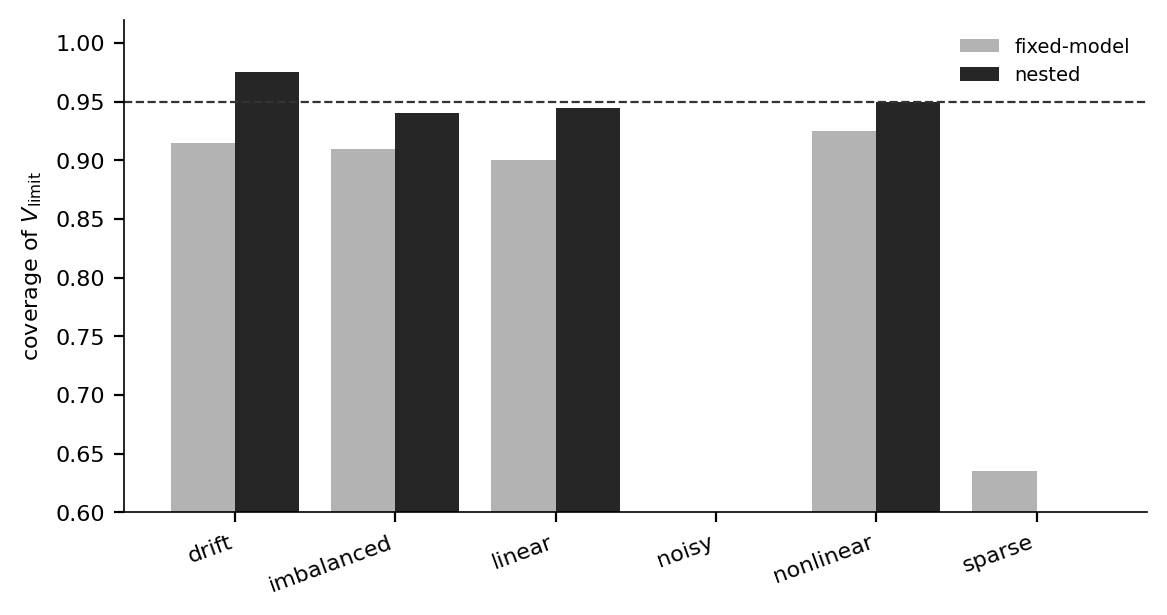
\includegraphics[width=0.9\linewidth]{figS6_coverage.png}
\caption{Coverage of the estimator's own limit in \nWorlds\ simulated worlds,
by interval construction, with Monte Carlo error bars. The dashed line is
nominal. The fixed-model percentile interval is the conventional one; the
nested basic interval is the one this paper reports. The sparse world is where
they disagree by more than a few points, and the nested percentile bar there
is the failure the basic construction repairs.}
\label{fig:coverage}
\end{figure}

\begin{table}[t]
\centering
\small
\resizebox{\ifdim\width>\linewidth\linewidth\else\width\fi}{!}{%%
\begin{tabular}{lrrrrrrrrr}
\toprule
world & bias vs limit & width (basic) & fixed pct & fixed basic & fixed bc & nested pct & nested basic & nested bc & m-out-of-n \\
\midrule
drift & 0.000 & 0.037 & 0.919 & 0.917 & 0.914 & 0.966 & 0.919 & 0.920 & -- \\
imbalanced & $-$0.010 & 0.116 & 0.906 & 0.906 & 0.900 & 0.933 & 0.933 & 0.923 & -- \\
linear & $-$0.002 & 0.060 & 0.925 & 0.931 & 0.915 & 0.939 & 0.931 & 0.921 & 0.768 \\
noisy & $-$0.002 & 0.036 & 0.926 & 0.924 & 0.916 & 0.936 & 0.948 & 0.939 & -- \\
nonlinear & $-$0.002 & 0.044 & 0.923 & 0.923 & 0.924 & 0.940 & 0.929 & 0.929 & 0.758 \\
sparse & $-$0.012 & 0.034 & 0.631 & 0.643 & 0.620 & 0.372 & 0.899 & 0.631 & 0.728 \\
\bottomrule
\end{tabular}%
}
\caption{Coverage of the estimator's own limit $V_{\mathrm{limit}}$ in each simulated world, under seven interval constructions, at the replicate count of Section~\ref{sec:sim}, with the estimator's bias against that limit and the mean width of the interval this paper reports. Nominal is $0.95$; the Monte Carlo standard error on a coverage is \simCoverageSE\ percentage points, so differences below about a point are not differences. An empty cell is a construction not priced on that world.}
\label{tab:sim31}
\end{table}


\begin{table}[t]
\centering
\small
\resizebox{\ifdim\width>\linewidth\linewidth\else\width\fi}{!}{%%
\begin{tabular}{llrrrrlr}
\toprule
n train & K & basic coverage & pct coverage & basic mean width & pct mean width & replicates & coverage se (pp) \\
\midrule
2000 & 20 & 0.887 & 0.887 & 0.085 & 0.085 & 150 & 2.588 \\
2000 & 200 & 0.780 & 0.480 & 0.042 & 0.042 & 150 & 3.382 \\
2000 & 1000 & 0.453 & 0.100 & 0.064 & 0.064 & 150 & 4.065 \\
4000 & 20 & 0.900 & 0.907 & 0.057 & 0.057 & 150 & 2.449 \\
4000 & 200 & 0.907 & 0.500 & 0.031 & 0.031 & 150 & 2.375 \\
4000 & 1000 & 0.507 & 0.080 & 0.047 & 0.047 & 150 & 4.082 \\
8000 & 20 & 0.893 & 0.900 & 0.039 & 0.039 & 150 & 2.520 \\
8000 & 200 & 0.893 & 0.480 & 0.021 & 0.021 & 150 & 2.520 \\
8000 & 1000 & 0.613 & 0.033 & 0.034 & 0.034 & 150 & 3.976 \\
8000 & 3019 & 0.213 & 0.000 & 0.026 & 0.026 & 150 & 3.345 \\
\bottomrule
\end{tabular}%
}
\caption{Sample size and register cardinality varied jointly. Coverage of $V_{\mathrm{limit}}$ and mean interval width for the nested percentile and the nested basic construction. The last row is the cardinality regime of the case study's own register. \emph{How well these are determined.} Every cell is \simGridReps\ replicates, not the \simCoreReps\ of the core experiment, and the coverages here are far from nominal --- so the Monte Carlo standard error of a coverage in this table has a median of \simGridSEMedian\ percentage points and reaches \simGridSEMax, against the \simCoverageSE\ that Section~\ref{sec:simsensitivity} quotes for the core. It is \simGridSERatio\ times larger, it is computed at each cell's own observed rate rather than at the nominal one, and it is a column here rather than a sentence because the differences down this table are read row against row.}
\label{tab:sim31grid}
\end{table}


\begin{table}[t]
\centering
\small
\resizebox{\ifdim\width>\linewidth\linewidth\else\width\fi}{!}{%%
\begin{tabular}{lrrr}
\toprule
world & block multiplier & nested basic & nested pct \\
\midrule
linear & 0.500 & 0.896 & 0.944 \\
linear & 1.000 & 0.920 & 0.908 \\
linear & 2.000 & 0.916 & 0.932 \\
sparse & 0.500 & 0.856 & 0.392 \\
sparse & 1.000 & 0.836 & 0.332 \\
sparse & 2.000 & 0.872 & 0.408 \\
\bottomrule
\end{tabular}%
}
\caption{Three block lengths around $n^{1/3}$: the multiplier column is the factor applied to the rule of thumb, so $0.5$ halves the block and $2$ doubles it. Coverage of $V_{\mathrm{limit}}$.}
\label{tab:sim31block}
\end{table}


\begin{table}[t]
\centering
\small
\resizebox{\ifdim\width>\linewidth\linewidth\else\width\fi}{!}{%%
\begin{tabular}{llllrrrrrr}
\toprule
family & draws are & K & draws & multiplier & mult., MC upper & empirical & emp., OS upper & Rademacher & per-cell \\
\midrule
decision-curve & degenerate & 248 & 200 & 0.803 & 0.805 & 0.935 & 0.964 & 0.785 & 0.937 \\
decision-curve & degenerate & 1100 & 400 & 0.929 & 0.930 & 0.948 & 0.962 & 0.773 & 0.940 \\
decision-curve & gaussian & 248 & 200 & 0.932 & 0.933 & 0.918 & 0.959 & 0.921 & 0.941 \\
decision-curve & gaussian & 1100 & 400 & 0.932 & 0.936 & 0.920 & 0.954 & 0.925 & 0.945 \\
decision-curve & heavy & 248 & 200 & 0.912 & 0.914 & 0.936 & 0.961 & 0.900 & 0.940 \\
decision-curve & heavy & 1100 & 400 & 0.913 & 0.915 & 0.938 & 0.955 & 0.904 & 0.944 \\
decision-curve & nonzero & 248 & 200 & 0.903 & 0.906 & 0.932 & 0.964 & 0.889 & 0.940 \\
decision-curve & nonzero & 1100 & 400 & 0.921 & 0.921 & 0.943 & 0.957 & 0.915 & 0.946 \\
whole-surface & degenerate & 180 & 400 & 0.923 & 0.924 & 0.945 & 0.966 & 0.920 & 0.946 \\
whole-surface & gaussian & 180 & 400 & 0.943 & 0.945 & 0.936 & 0.959 & 0.936 & 0.946 \\
whole-surface & heavy & 180 & 400 & 0.915 & 0.919 & 0.947 & 0.967 & 0.913 & 0.945 \\
whole-surface & nonzero & 180 & 400 & 0.925 & 0.927 & 0.946 & 0.971 & 0.920 & 0.946 \\
\bottomrule
\end{tabular}%
}
\caption{Family-wise coverage of the max-$t$ band against a known answer, over synthetic families matched to this corpus in size, cross-cell correlation and per-cell excess kurtosis, and spanning draw counts around the one it runs. EVERY ROW IS A FAMILY THE CORPUS RUNS: \textsf{whole-surface} at $K = \nCellsPerPairMedian$ and \nDrawsSurface\ draws is every pair's surface family, \textsf{decision-curve} at $K = \nDcaFamilyModal$ and \nDrawsSurface\ draws the modal curve family, and the \nDcaFamily-cell row at \nDcaDraws\ draws the case study's own curve family; the draw-count ladder the text quotes is a sensitivity around the first and is not printed here. Nominal is $0.95$; the five middle columns are the five candidate critical values and the last is the control. \emph{The bootstrap here is ideal} --- the draws come from the sampling distribution itself --- so every coverage in this table is an upper bound on what the real procedure attains, and the control says why: \emph{per-cell} is the basic interval the band is built from, on the same draws, and it is short of nominal before any multiplicity correction is applied. \emph{Regimes.} \textsf{gaussian} is the case the multiplier bootstrap is derived for; \textsf{heavy} carries this corpus's measured tails; \textsf{degenerate} adds the cells whose net-benefit difference is zero by arithmetic, which the corpus's decision-curve families contain and its surface families do not; \textsf{nonzero} is heavy with a fixed heterogeneous non-zero truth, the regime under which a cell can be resolved correctly and a region label is actually being asked to hold. Every cell is \nBandCoverageReps\ replicates, so no coverage here is determined worse than \bandCoverageSEMax.}
\label{tab:bandcov}
\end{table}


\begin{table}[t]
\centering
\small
\resizebox{\ifdim\width>\linewidth\linewidth\else\width\fi}{!}{%%
\begin{tabular}{lllrlrrrrrrr}
\toprule
world & n train & K & K / n & replicates & coverage at c = 1 & se & c & c lo & c hi & c applied & c log-linear \\
\midrule
linear & 180000 & 200 & 0.001 & 500 & 0.882 & 0.014 & 1.352 & 1.174 & 1.482 & 1.177 & 1.000 \\
linear & 8000 & 20 & 0.003 & 500 & 0.916 & 0.012 & 1.154 & 1.073 & 1.307 & 1.177 & 1.000 \\
linear & 4000 & 20 & 0.005 & 500 & 0.898 & 0.014 & 1.219 & 1.101 & 1.313 & 1.177 & 1.056 \\
linear & 2000 & 20 & 0.010 & 500 & 0.924 & 0.012 & 1.108 & 1.024 & 1.228 & 1.177 & 1.134 \\
linear & 50000 & 625 & 0.013 & 498 & 0.902 & 0.013 & 1.296 & 1.135 & 1.689 & 1.177 & 1.160 \\
linear & 8000 & 100 & 0.013 & 500 & 0.936 & 0.011 & 1.096 & 0.960 & 1.203 & 1.177 & 1.160 \\
sparse & 8000 & 100 & 0.013 & 500 & 0.892 & 0.014 & 1.317 & 1.220 & 1.453 & 1.177 & 1.160 \\
linear & 2000 & 25 & 0.013 & 500 & 0.908 & 0.013 & 1.188 & 1.072 & 1.277 & 1.177 & 1.160 \\
linear & 750 & 10 & 0.013 & 500 & 0.920 & 0.012 & 1.117 & 1.029 & 1.207 & 1.177 & 1.168 \\
linear & 4000 & 100 & 0.025 & 500 & 0.896 & 0.014 & 1.179 & 1.087 & 1.296 & 1.177 & 1.245 \\
linear & 8000 & 200 & 0.025 & 499 & 0.932 & 0.011 & 1.093 & 0.985 & 1.264 & 1.177 & 1.245 \\
sparse & 4000 & 200 & 0.050 & 500 & 0.884 & 0.014 & 1.182 & 1.131 & 1.299 & 1.177 & 1.337 \\
linear & 2000 & 100 & 0.050 & 500 & 0.912 & 0.013 & 1.234 & 1.055 & 1.326 & 1.177 & 1.337 \\
linear & 4000 & 200 & 0.050 & 500 & 0.888 & 0.014 & 1.195 & 1.119 & 1.337 & 1.177 & 1.337 \\
linear & 8000 & 400 & 0.050 & 500 & 0.884 & 0.014 & 1.152 & 1.104 & 1.226 & 1.177 & 1.337 \\
linear & 750 & 38 & 0.051 & 500 & 0.926 & 0.012 & 1.103 & 0.989 & 1.259 & 1.177 & 1.338 \\
sparse & 2000 & 200 & 0.100 & 500 & 0.836 & 0.017 & 1.333 & 1.224 & 1.372 & 1.310 & 1.435 \\
linear & 500 & 50 & 0.100 & 500 & 0.874 & 0.015 & 1.250 & 1.141 & 1.460 & 1.310 & 1.435 \\
linear & 4000 & 400 & 0.100 & 499 & 0.796 & 0.018 & 1.287 & 1.221 & 1.399 & 1.310 & 1.435 \\
linear & 2000 & 200 & 0.100 & 500 & 0.844 & 0.016 & 1.316 & 1.253 & 1.417 & 1.310 & 1.435 \\
linear & 8000 & 1000 & 0.125 & 496 & 0.655 & 0.021 & 1.526 & 1.417 & 1.600 & 1.441 & 1.468 \\
linear & 2000 & 250 & 0.125 & 500 & 0.792 & 0.018 & 1.404 & 1.284 & 1.485 & 1.441 & 1.468 \\
linear & 750 & 94 & 0.125 & 500 & 0.872 & 0.015 & 1.310 & 1.154 & 1.396 & 1.441 & 1.468 \\
linear & 2000 & 400 & 0.200 & 500 & 0.758 & 0.019 & 1.562 & 1.398 & 1.670 & 1.562 & 1.540 \\
sparse & 4000 & 1000 & 0.250 & 498 & 0.460 & 0.022 & 1.716 & 1.672 & 1.849 & 1.727 & 1.575 \\
linear & 4000 & 1000 & 0.250 & 500 & 0.520 & 0.022 & 1.739 & 1.632 & 1.805 & 1.727 & 1.575 \\
linear & 8000 & 3019 & 0.377 & 488 & 0.305 & 0.021 & 1.881 & 1.804 & 1.988 & 1.791 & 1.643 \\
linear & 500 & 200 & 0.400 & 500 & 0.760 & 0.019 & 1.450 & 1.353 & 1.656 & 1.791 & 1.653 \\
linear & 2000 & 1000 & 0.500 & 500 & 0.462 & 0.022 & 1.869 & 1.788 & 2.024 & 1.869 & 1.691 \\
\bottomrule
\end{tabular}%
}
\caption{The coverage calibration. For each cell of the $(n, K)$ plane: the coverage the reported interval actually attains, and the factor $c$ by which it must be widened to attain the nominal level, with the Monte Carlo interval of that factor. $c$ is the $0.95$ quantile of the studentised error and is computed, not searched for. `c applied' is the monotone regression the corpus is calibrated with; `c log-linear' is the parametric fit whose slope Section~\ref{sec:regions} quotes, printed beside it because it sits below the measured factor at small ratios and would under-correct there.}
\label{tab:plane}
\end{table}

